%KASCADE gamma search

% \begin{frame}{KASCADE-Grande}
% \begin{itemize}
%   \item Proposed in 1989---disassembled in 2013;
%   \item Aimed at studying
%   high-evergy (galactic) cosmic rays by observing extensive air showers (EAS);
% %   processes at the edge of the Galaxy and beyond by observing extended atmospheric showers (EAS);
%   \item Consisted of:
%   \begin{itemize}
%     \item scintillators detecting $e$, $\gamma$, $\mu$:
%     \begin{itemize}
%   %сцинтиляторы, различают e, gamma, mu
%     \item KASCADE---256 stations;
%     \item GRANDE---37 stations;
%     \end{itemize}
%  %один большой калориметр
%     \item Hadronic callorimeter;
%  %радиодетектор
%     \item Digital radio array LOPES detecting $e$, $e^{+}$;
% % позволяющих наблюдать различные компоненты ливня
%   \end{itemize}
%   \item Important features of cosmic-ray spectrum have been obtained. The data analysis is ongoing;
% %  благодаря данным с эксперимента было открыто много всего ополезного, при этом анлиз данных продолжается. новые статьи выходят
%   \item KCDC (\textbf{K}ASCADE \textbf{C}osmic Ray \textbf{D}ata \textbf{C}enter, \textcolor{blue}{\texttt{http://kcdc.ikp.kit.edu}}) is a dedicated portal where all the data collected are available online. % At the moment
% \end{itemize}
%
% \begin{frame}{KASCADE-Grande gamma-ray limits}
% %   \item Limits on the ratio of diffuse gamma-ray flux to cosmic ray flux
%   \begin{minipage}{0.5\textwidth}
%    left
%   \end{minipage}
%
% %   \begin{columns}
% %     \column{0.5\textwidth}
% %     left
% %     \column{0.5\textwidth}
% %     right
% %   \end{columns}
% \end{frame}


\section{KASCADE \texorpdfstring{$\gamma$}{gamma}-ray search}

\begin{frame}{HAWC highest-energy $\gamma$-ray sources}

\begin{itemize}
  \item six sources in the Galactic plane that emit above 56~TeV:
\end{itemize}
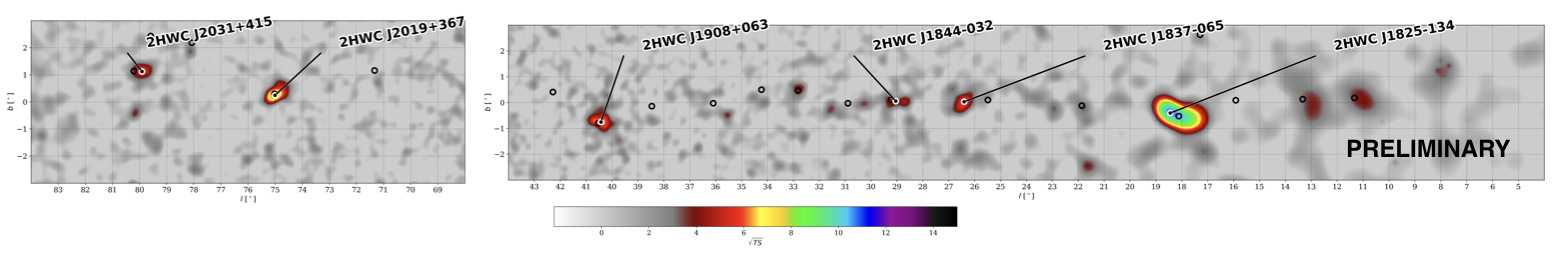
\includegraphics[width=1\textwidth]{pics/HWC_above_56TeV.png}
\begin{itemize}
  \item two of them continue to emit past 100~TeV:
\end{itemize}
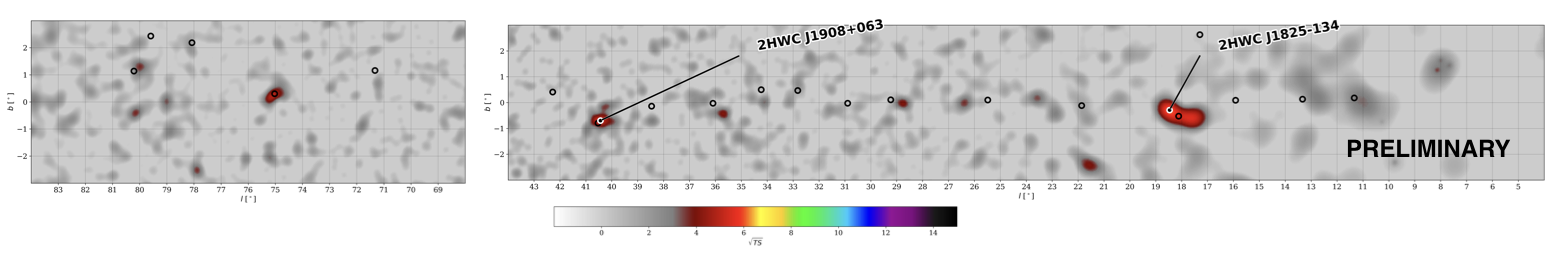
\includegraphics[width=1\textwidth]{pics/HWC_above_100TeV.png}

\small
[1] Malone, K. (2018). \textit{A survey of the highest-energy astrophysical sources with the HAWC Observatory (Doctoral dissertation)}.
Retrieved from https://hawc-observatory.org/publications/docs/Malone-Dissertation.pdf

\end{frame}

\begin{frame}{Sources in KASCADE field of view}
%   KASCADE data: Efficiency of registration, exposure map *
\begin{minipage}[c]{0.73\textwidth}
\begin{center}
  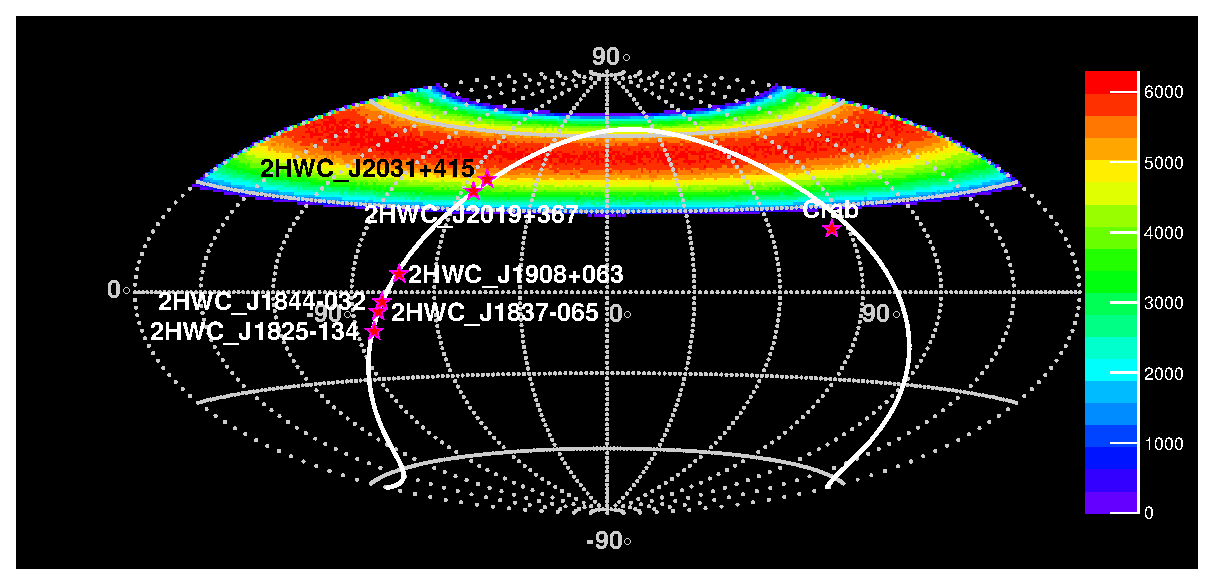
\includegraphics[width=1\textwidth]{pics/Skymap_6srcs.eps}\\
  KASCADE event distribution map\\
  with 6 HAWC sources\\
  with energy $E$ above 56~TeV.
\end{center}
\end{minipage}
\hfill
\begin{minipage}[c]{0.25\textwidth}
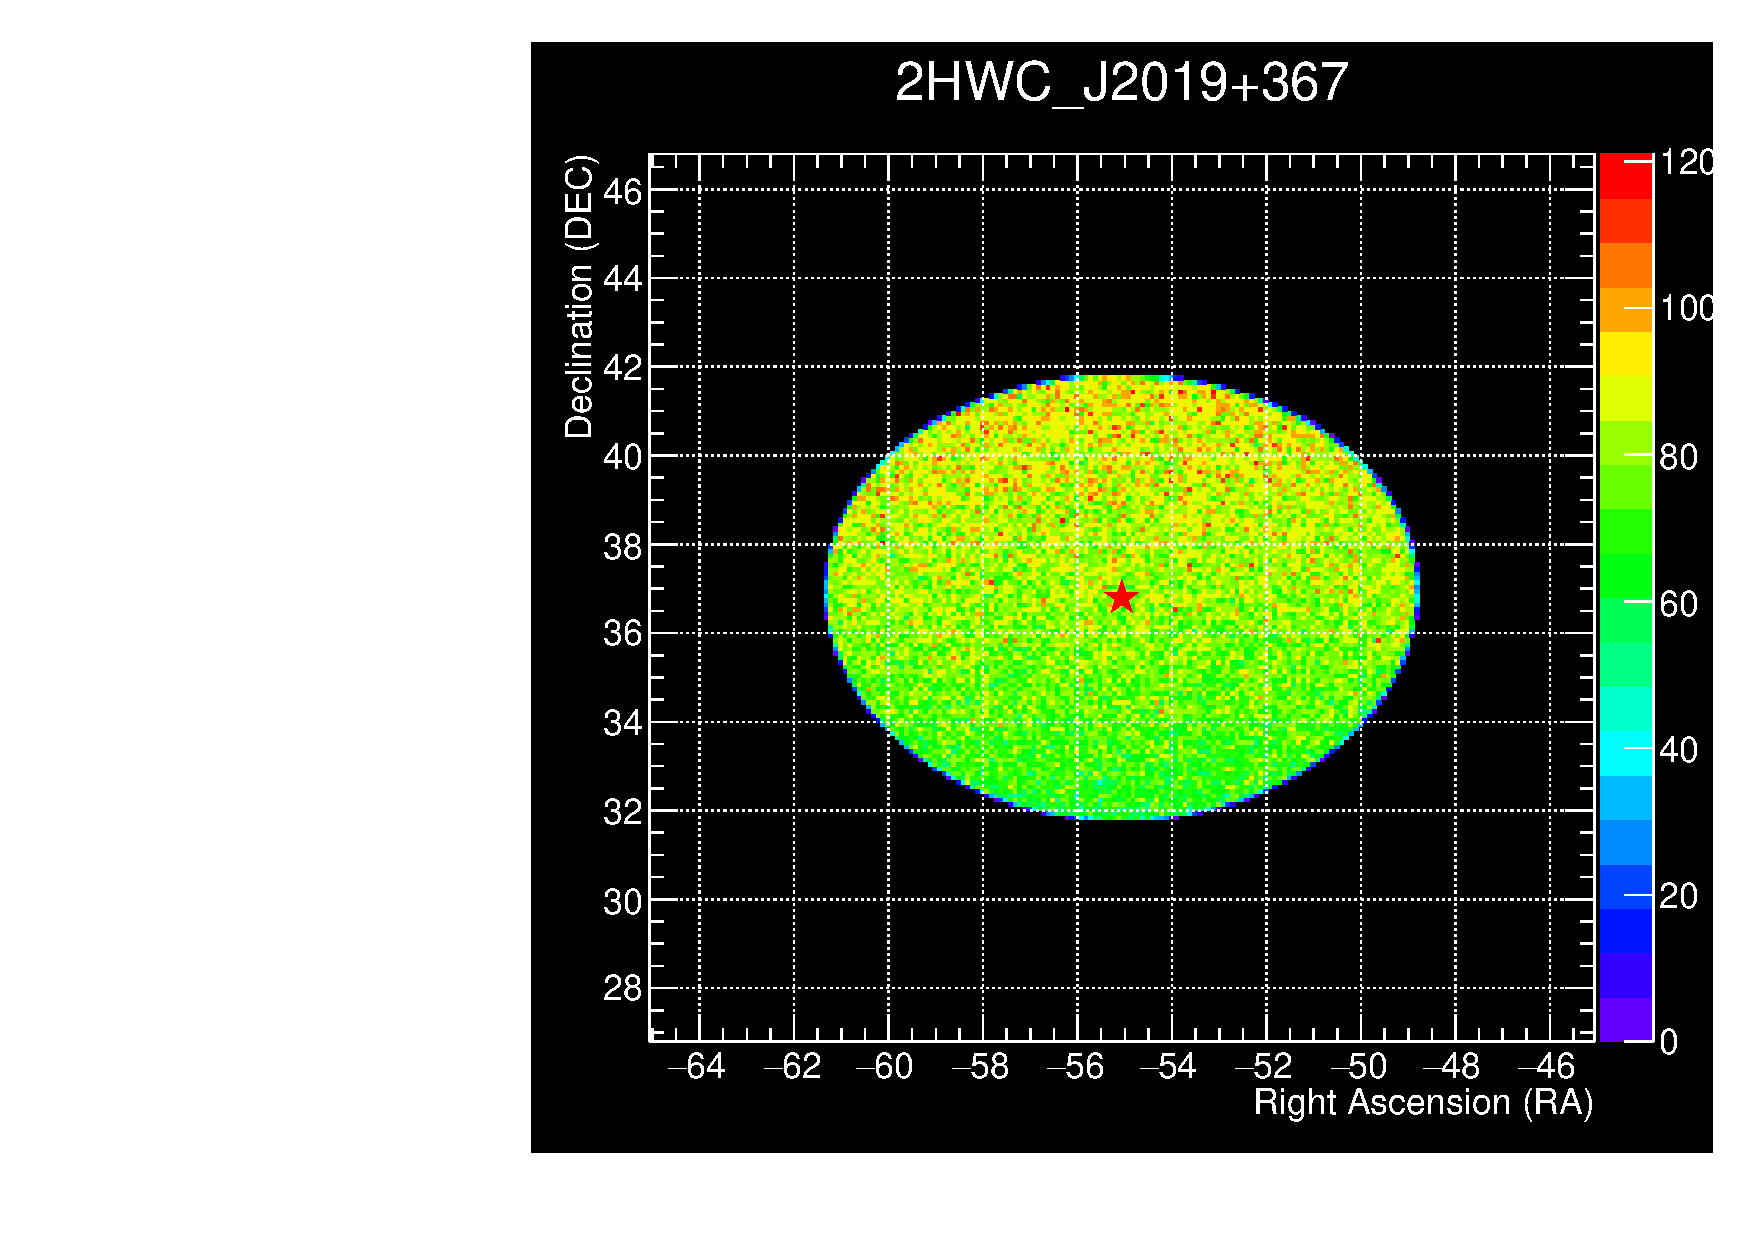
\includegraphics[width=1\textwidth]{pics/Skymap_2HWC_J2019+367.pdf}\\
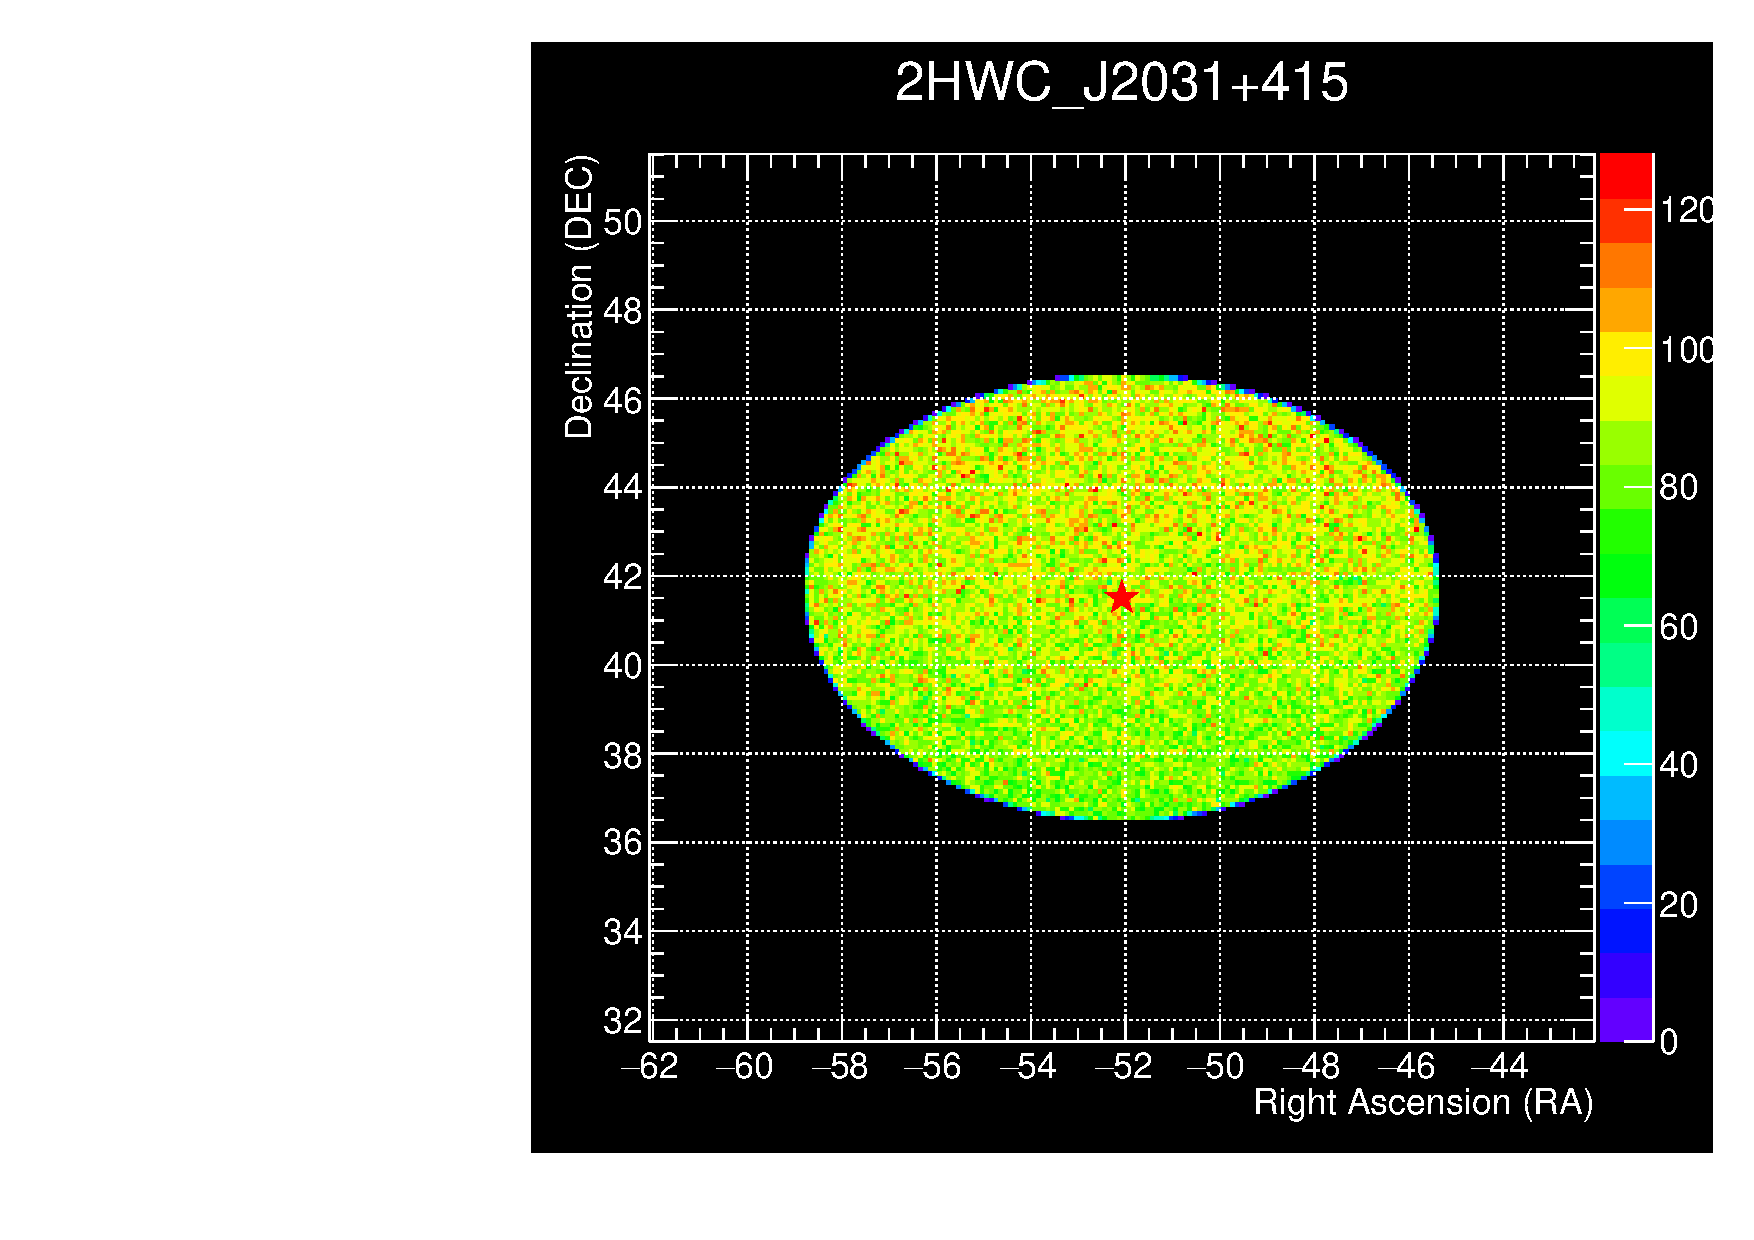
\includegraphics[width=1\textwidth]{pics/Skymap_2HWC_J2031+415.pdf}
\end{minipage}
\end{frame}

\begin{frame}{Data cuts and corrections}
\begin{center}
  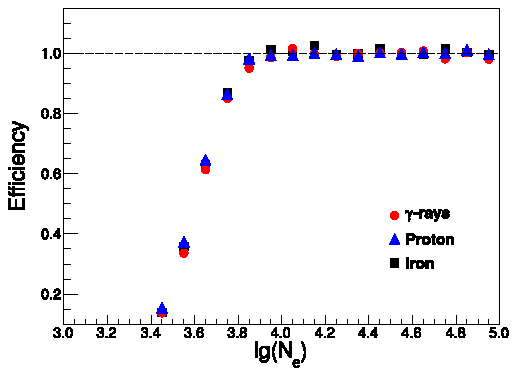
\includegraphics[height=0.39\textheight]{pics/eff_Ne_Donghwa.pdf}\hspace{1em}
  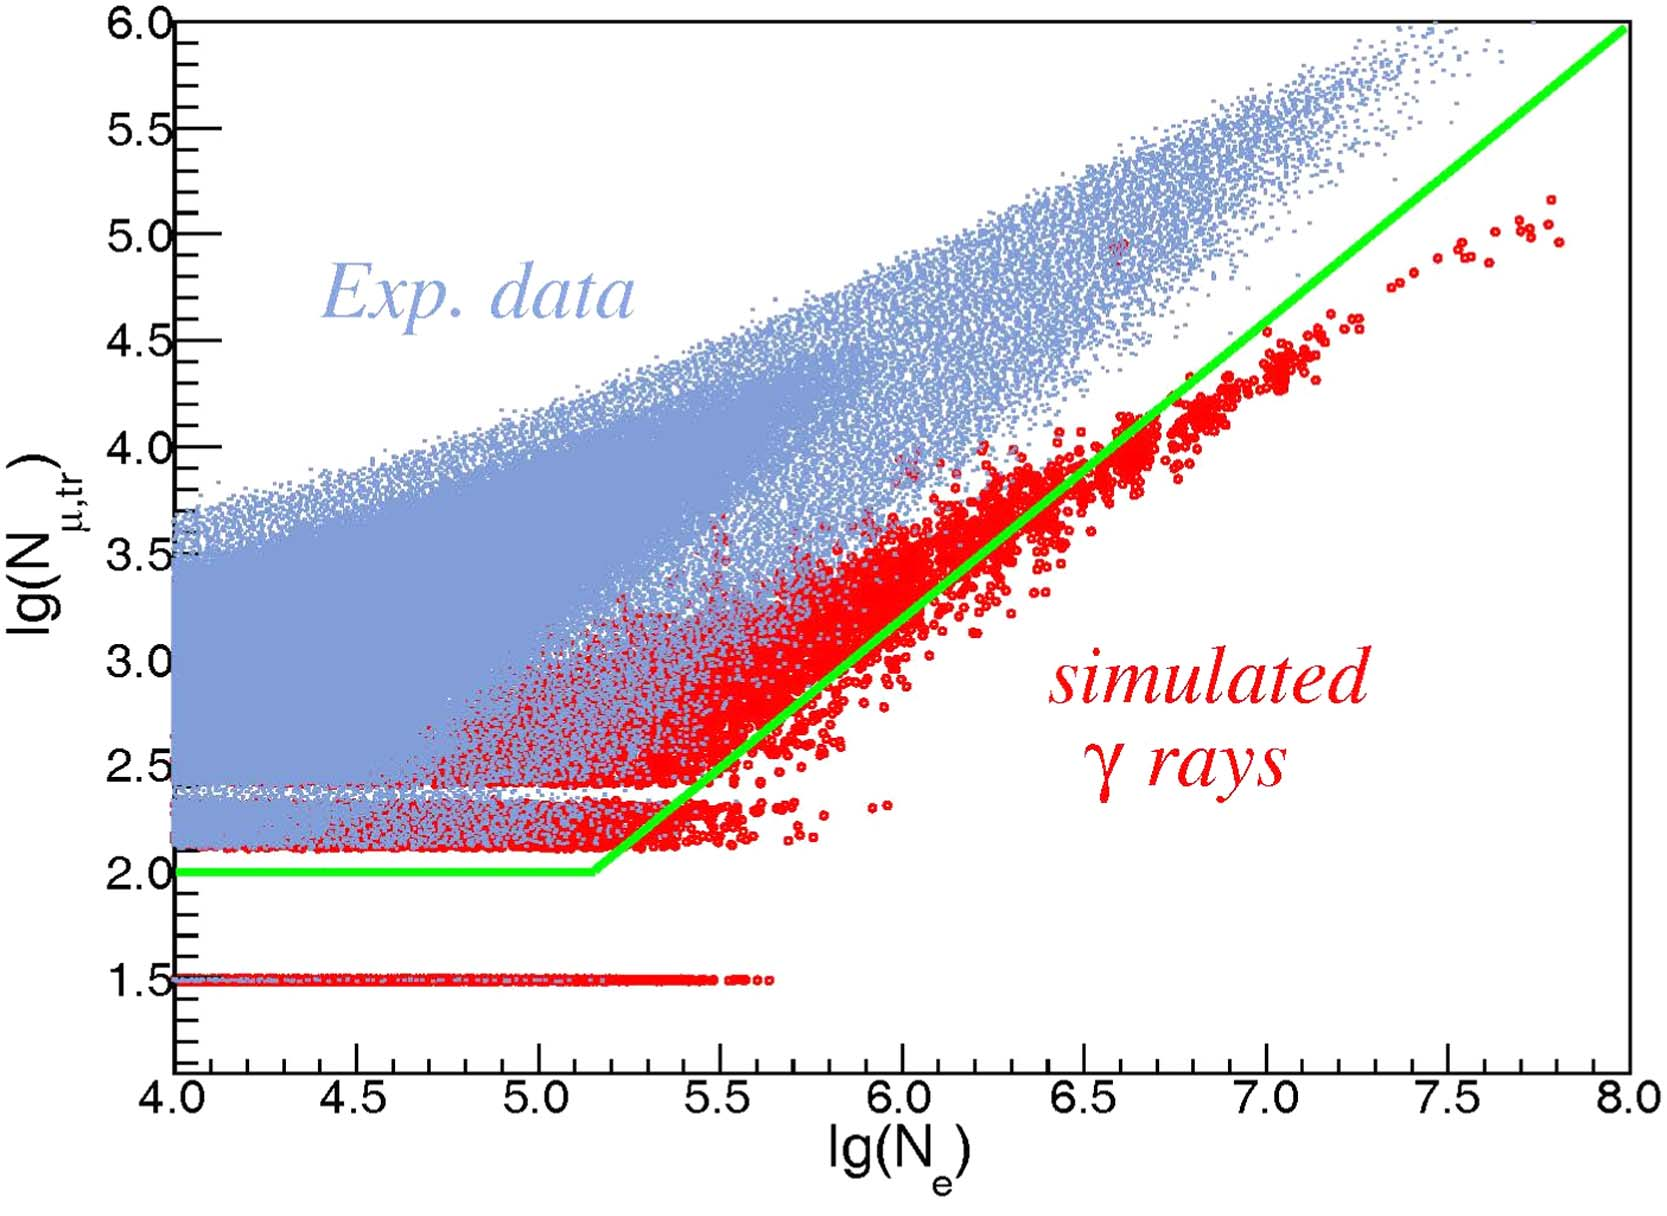
\includegraphics[height=0.39\textheight]{pics/gamma_cut.png}\\
  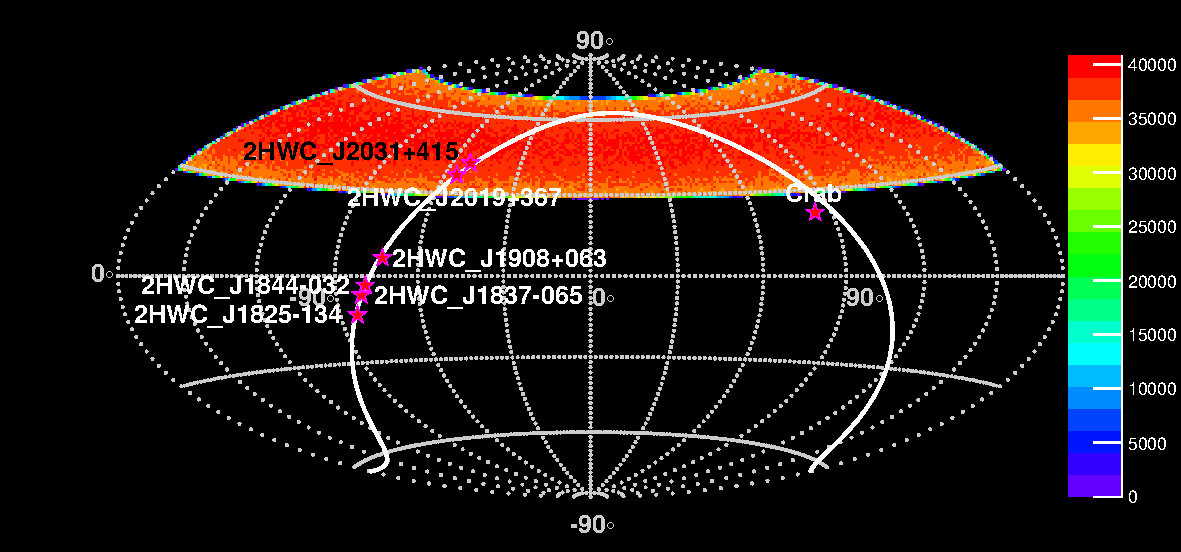
\includegraphics[height=0.42\textheight]{pics/Skymap_6srcs_exp.pdf}
\end{center}
\end{frame}

\begin{frame}{Estimation of the integral flux and the expected number of measured $\gamma$s for the \textit{2HWC\_J2013+415} source}
% \Large
\vspace{-3ex}
\[
F_\mathsf{int}(E) = \int_{E}^{\infty}F_0\left(\frac{E}{E_0}\right)^{\!\!-\alpha}d\alpha,
\]
\[
F_0 = 3.4\times10^{-14}~\mathsf{cm}^{-2} \mathsf{s}^{-1} \mathsf{TeV}^{-1},~
E_0 = 7~\mathsf{TeV},~
\alpha = 2.7.
\]

% \Large
\vspace{-1ex}
\[
\begin{array}{ccc}
E~[\mathsf{TeV}] & F_\mathsf{int}~[\mathsf{cm}^{-2}\mathsf{s}^{-1}] & N_\gamma (expected) \\\hline
7  & 1.4\times10^{-13} & 441\\
56  & 4.1\times10^{-15} & 12.9\\
100 & 1.5\times10^{-15} & 4.8 \\
1000 & 3.1\times10^{-17} & 0.096\\
\end{array}
\]

\vspace{0.4ex}
\normalsize
With $\alpha \approx -2.7$ KASCADE can have few gamma events with $E > 100$ TeV in dataset, though very close to the threshold. 

% At least up to 100~TeV the expected event numbers are in the range of sensitivity, though very close to the threshold. 

We need more statistics.
% There supposed to be 2 slides on this
%  Оценка количества событий вокруг 2HWC_J2013+415 +-
\end{frame}
